\documentclass{article}
\usepackage[utf8]{inputenc}
\usepackage{mathtools, mathrsfs, amsmath, amsthm,amssymb}
\usepackage[table]{xcolor}

\usepackage{tikz}
\usetikzlibrary{arrows}

\newenvironment{exercise}
{\noindent \subsubsection{}}
{}

\title{Multivariable Mathematics Solutions Manual}
\author{Thomas Hughes}
\date{November 2019}

\usepackage[pdfencoding=auto, psdextra]{hyperref}
\begin{document}

\maketitle

\tableofcontents

\newpage
\section{VECTORS AND MATRICES}
\subsection{Vectors in $\mathbb{R}^n$}

\begin{exercise} \label{e1.1.1}
    Given \( \mathbf{x} = \begin{bmatrix} 2 \\ 3 \end{bmatrix} \) and \( \mathbf{y} = \begin{bmatrix} -1 \\ 1 \end{bmatrix} \) calculate the following both algebraically and geometrically.
    \begin{enumerate}
        \item \( \mathbf{x}+\mathbf{y} \)
        \item \( \mathbf{x}-\mathbf{y} \)
        \item \( \mathbf{x}+2\mathbf{y} \)
        \item \( \frac{1}{2}\mathbf{x}+\frac{1}{2}\mathbf{y} \)
        \item \( \mathbf{y}-\mathbf{x} \)
        \item \( 2\mathbf{x}-\mathbf{y} \)
        \item \( \left\lVert \mathbf{x} \right\rVert \)
        \item \( \frac{\mathbf{x}}{\left\lVert \mathbf{x} \right\rVert} \)
    \end{enumerate}
    
    \begin{proof}
        \begin{enumerate}
            \item \( \mathbf{x}+\mathbf{y}=\begin{bmatrix} 2 \\ 3 \end{bmatrix} + \begin{bmatrix} -1 \\ 1 \end{bmatrix} = \begin{bmatrix} 2+(-1) \\ 3 + 1 \end{bmatrix} = \begin{bmatrix} 1 \\ 4 \end{bmatrix} \)
        \end{enumerate}
        
        The idea is similar for the rest.
    \end{proof}
\end{exercise}

\begin{exercise} \label{e1.1.2}
    Three vertices of a parallelogram are \( \begin{bmatrix} 1 \\ 2 \\ 1 \end{bmatrix}, \begin{bmatrix} 2 \\ 4 \\ 3 \end{bmatrix},\text{ and } \begin{bmatrix} 3 \\ 1 \\ 5 \end{bmatrix} \). What are all the possible positions of the fourth vertex? Give your reasoning.
    
    \begin{proof}
        The three vertices given already define a plane, which implies that any fourth vertex would have to belong to the plane as well. Thus the problem is reduced to finding the three points in the plane that will produce a parallelogram. Each solution is given by the sum of the three original vectors where one of them is negative. The three points then are given by:
        \begin{align*}
            \begin{bmatrix} 1 \\ 2 \\ 1 \end{bmatrix} + \begin{bmatrix} 2 \\ 4 \\ 3 \end{bmatrix} - \begin{bmatrix} 3 \\ 1 \\ 5  \end{bmatrix} &= \begin{bmatrix} 0 \\ 5 \\ -1 \end{bmatrix} \\
            \begin{bmatrix} 2 \\ 4 \\ 3 \end{bmatrix} + \begin{bmatrix} 3 \\ 1 \\ 5 \end{bmatrix} - \begin{bmatrix} 1 \\ 2 \\ 1 \end{bmatrix} &= \begin{bmatrix} 4 \\ 3 \\ 7 \end{bmatrix} \\
            \begin{bmatrix} 3 \\ 1 \\ 5 \end{bmatrix} + \begin{bmatrix} 1 \\ 2 \\ 1 \end{bmatrix} - \begin{bmatrix} 2 \\ 4 \\ 3 \end{bmatrix} &= \begin{bmatrix} 2 \\ -1 \\ 3 \end{bmatrix} \\
        \end{align*}
        
        \begin{center}
            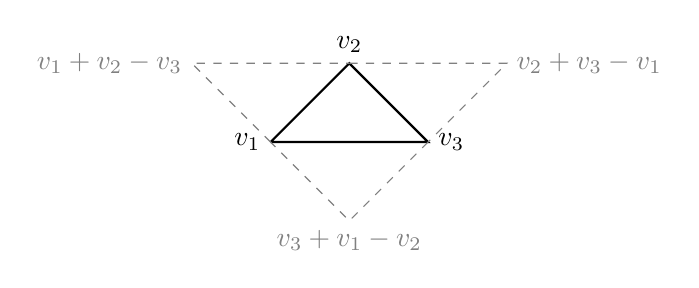
\begin{tikzpicture}
                \draw[thick] (-1,0) node[anchor=east] {$v_1$}
                -- (0,1) node[anchor=south] {$v_2$}
                -- (1,0) node[anchor=west] {$v_3$}
                -- (-1,0);
                
                \draw[color=gray,dashed] (0,1)
                -- (2,1) node[anchor=west] {$v_2+v_3-v_1$}
                -- (1,0);
                
                \draw[color=gray,dashed] (1,0)
                -- (0,-1) node[anchor=north] {$v_3+v_1-v_2$}
                -- (-1,0);
                
                \draw[color=gray,dashed] (-1,0)
                -- (-2,1) node[anchor=east] {$v_1+v_2-v_3$}
                -- (0,1);
            \end{tikzpicture}
        \end{center}
    \end{proof}
\end{exercise}

\begin{exercise} \label{e1.1.3}
    The origin is at the center of a regular polygon.
    \begin{enumerate}
        \item What is the sum of the vectors to each of the vertices of the polygon? Give your reasoning.
        \item What is the sum of the vectors from one fixed vertex to each of the remaining vertices? Give your reasoning
    \end{enumerate}
    
    \begin{proof}
        \begin{enumerate}
            \item Let one of the vertices of the polygon be at \( (r,0) \), where \(r>0\). By symmetry of the polygon, it follows that the sum of all the \(y\)-components of the vectors is \( 0 \). One can use the identity
            \[
            \sum_{k=0}^{n-1} \cos(a+kd) = \cos\left( \frac{a+(n-1)d}{2} \right)\frac{ \sin\left( n \frac{d}{2} \right) }{\sin\left( \frac{d}{2} \right)}
            \]
            to show that the \(x\)-components of the vectors sum to \( 0 \). Thus the sum of the vectors is \( \mathbf{0} \).
            
            \item Let \( v_i \) denote the vector from the origin to the \( i^{th} \) vertex, where the vector from the center to the source vertex is \( v_1 \). Let \( w_i \) denote the vector from the source vertex to the \( i^{th} \) vertex. Then \( w_i = v_i - v_1 \). Thus
            
            \begin{align*}
                \sum_{i=2}^n w_i &= \sum_{i=2}^n (v_i - v_1) \\
                &= \sum_{i=2}^n v_i - (n-1)v_1 \\
                \intertext{and by the previous problem}
                &= -nv_1
            \end{align*}
        \end{enumerate}
    \end{proof}
\end{exercise}

\begin{exercise} \label{e1.1.4}
    Given \( \triangle ABC \), let \( M \) and \( N \) denote the midpoints of \( \overline{AB} \) and \( \overline{AC} \), respectively. Prove that \( \overrightarrow{MN} = \frac{1}{2} \overrightarrow{BC} \).
    
    \begin{proof}
        Set \( A = (0,0) \). Then
            \begin{align*}
                \overrightarrow{M} &= \frac{1}{2}\overrightarrow{AB} \\
                \overrightarrow{N} &= \frac{1}{2}\overrightarrow{AC} \\
                \intertext{So that}
                \overrightarrow{MN} &= \overrightarrow{M}-\overrightarrow{N} \\
                &= \frac{1}{2}\overrightarrow{AB} - \frac{1}{2}\overrightarrow{AC} \\
                &= \frac{1}{2} \left( \overrightarrow{AB}-\overrightarrow{AC} \right) \\
                &= \frac{1}{2} \overrightarrow{BC}
            \end{align*}
            \begin{center}
                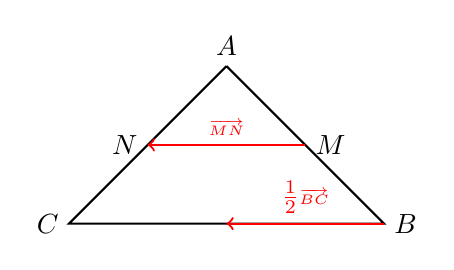
\begin{tikzpicture}
                    \draw[thick] (0,1) node[anchor=south] {$A$}
                    --(1,0) node[anchor=west] {$M$}
                    --(2,-1) node[anchor=west] {$B$}
                    --(-2,-1) node[anchor=east] {$C$}
                    --(-1,0) node[anchor=east] {$N$}
                    --(0,1);
                    
                    \draw[red,thick,->] (1,0) -- (-1,0);
                    \draw[red] (0,0) node[anchor=south] {$\tiny{\overrightarrow{MN}}$};
                    
                    \draw[red,thick,->] (2,-1) -- (0,-1);
                    \draw[red] (1,-1) node[anchor=south] {$\tiny{\frac{1}{2}\overrightarrow{BC}}$};
                \end{tikzpicture}
            \end{center}
    \end{proof}
\end{exercise}

\begin{exercise} \label{e1.1.5}
    Let \( ABCD \) be an arbitrary quadrilateral. Let \( P,Q,R,\text{ and } S \) be the midpoints of \( \overline{AB},\overline{BC},\overline{CD},\text{ and } \overrightarrow{DA} \), respectively. Use vector methods to prove that \( PQRS \) is a parallelogram.
    
    \begin{proof}
        By the previous exercise, we know that
        \begin{alignat*}{3}
            \overrightarrow{SP} &= \frac{1}{2}\overrightarrow{DB} &= \overrightarrow{RQ}  \\
            \overrightarrow{PQ} &= \frac{1}{2}\overrightarrow{AC} &= \overrightarrow{SR} 
        \end{alignat*}
        implying that \( PQRS \) is a parallelgram.
        
        \begin{center}
            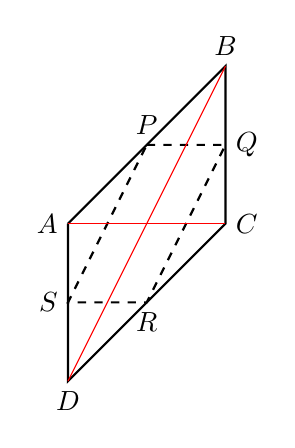
\begin{tikzpicture}
                \draw[thick] (0,0) node[anchor=east] {$A$}
                -- (1,1) node[anchor=south] {$P$}
                -- (2,2) node[anchor=south] {$B$}
                -- (2,1) node[anchor=west] {$Q$}
                --(2,0) node[anchor=west] {$C$}
                --(1,-1) node[anchor=north] {$R$}
                --(0,-2) node[anchor=north] {$D$}
                --(0,-1) node[anchor=east] {$S$}
                --(0,0);
                
                \draw[dashed,thick] (1,1)
                --(2,1)
                --(1,-1)
                --(0,-1)
                --(1,1);
                
                \draw[red] (0,-2)
                --(2,2);
                
                \draw[red] (0,0)
                --(2,0);
            \end{tikzpicture}
        \end{center}
    \end{proof}
\end{exercise}


\subsection{Dot Product}

\begin{exercise} \label{e1.2.1}
    For each of the following pairs of vectors \( x \) and \( y \), calculate \( x \cdot y \) and the angle \( \theta \) between the vectors.
    \[
    x=\begin{bmatrix}2\\5\end{bmatrix},y=\begin{bmatrix}-5\\2\end{bmatrix}
    \]
    \begin{proof}
        \[ x \cdot y = 2(-5)+5(2) = 0 \]
        and
        \[
        \theta = \cos^{-1}{\frac{x\cdot y}{\lVert x \rVert \lVert y \rVert}} = \frac{\pi}{2}
        \]
        The rest of the problems are similar.
    \end{proof}
\end{exercise} %1.2.1

\begin{exercise} \label{e1.2.2}
    For each pair of vectors in Exercise 1, calculate \( \text{proj}_{y}x \) and \( \text{proj}_{x}y \)
    
    \begin{proof}
        Since we saw that \( x \cdot y = 0 \), we have
        \[ \text{proj}_{x}y = \frac{x \cdot y}{\lVert x \rVert^2}x = \text{proj}_{y}x = \frac{x \cdot y}{\lVert y \rVert^2}y = 0 \]
        The remaining are similar.
    \end{proof}
\end{exercise} %e1.2.2

\begin{exercise} \label{e1.2.3}
    Find the angle between the long diagonal of a cube and a face diagonal.
    
    \begin{proof}
        Wlog, take the unit cube. Denote the long diagonal \( l = \begin{bmatrix} 1\\1\\1 \end{bmatrix} \) and, wlog, the short diagonal \( s = \begin{bmatrix} 0 \\ 1 \\ 1 \end{bmatrix} \). Then
        \[
        \theta = \cos^{-1}\frac{l \cdot s}{\lVert l \rVert \lVert s \rVert} = \frac{2}{\sqrt{3}\sqrt{2}} = \sqrt{\frac{2}{3}}
        \]
    \end{proof}
\end{exercise} %e1.2.3

\begin{exercise} \label{1.2.4}
    Find the angle that the long diagonal of a \( 3 \times 4 \times 5 \) rectangular box makes with the longest edge.
    
    \begin{proof}
        
    \end{proof}
\end{exercise} %e1.2.4

\begin{exercise} \label{e1.2.5}
    Suppose \( x, y \in \mathbb{R}^n \), \( \lVert x \rVert =2, \lVert y \rVert =1 \), and the angle \( \theta \) between \( x \) and \( y \) is \( \theta = \arccos{\frac{1}{4}} \). Prove that the vectors \( x-3y \) and \( x+y \) are orthogonal.

    \begin{proof}
        Since \( \theta = \arccos{\frac{1}{4}} \) it follows that
        \begin{align*}
        \frac{1}{4} = &\cos{\theta} = \frac{x \cdot y}{\lVert x \rVert \lVert y \rVert} \\
        \frac{1}{2} &= x \cdot y
        \end{align*}
        Thus
        \begin{align*}
            (x-3y) \cdot (x+y) &= (x \cdot x) + (x \cdot y) - 3(y \cdot x) + (y \cdot y)\\
            &= 4 - 2 (x \cdot y) -3 \\
            &= 0
        \end{align*}
    \end{proof}
\end{exercise} %e1.2.5

\begin{exercise} \label{e1.2.6}
    Suppose \( x,y,z \in \mathbb{R}^2 \) are unit vectors satisfying \( x+y+z=0 \). What can you say about the angles between each pair?
    
    \begin{proof}
        Note that, more generally, we have
        \[ \lVert x_1 \rVert = \lVert x_2 \rVert = \lVert x_3 \rVert = 1 \]
        and
        \[ x_3 = -x_1-x_2 \]
        Thus
        \begin{align*}
             0 &= (x_1+x_2+x_3) \cdot (x_1+x_2+x_3) \\
             &= 3 + 2\left((x_1 \cdot x_2) + (x_1 \cdot x_3) + (x_2 \cdot x_3)\right) \\
             &= 3 + 2\left( (x_1 \cdot x_2) + (x_1 \cdot (-x_1-x_2)) + (x_2 \cdot (-x_1-x_2)) \right) \\
             &= 3 + 2\left( (x_1 \cdot x_2) - 2 - 2(x_1 \cdot x_2) \right) \\
             &= 3 - 4 - 2(x_1 \cdot x_2) \\
             &= -1 - 2(x_1 \cdot x_2)
             \intertext{thus}
             -\frac{1}{2} &= x_1 \cdot x_2
        \end{align*}
        
        It therefore follows that the angle, \( \theta \), between any pair is given by
        \[ \theta = \arccos{-\frac{1}{2}} = \frac{2\pi}{3} \]
    \end{proof}
\end{exercise} %e1.2.6

\begin{exercise} \label{e1.2.7}
    Let \( e_1 = \begin{bmatrix} 1 \\ 0 \\ 0  \end{bmatrix} \), \( e_2 = \begin{bmatrix} 0 \\ 1 \\ 0  \end{bmatrix} \), and \( e_3 = \begin{bmatrix} 0 \\ 0 \\ 1  \end{bmatrix} \) be the so-called \emph{standard basis vectors} of \( \mathbb{R}^3 \). Let \( x \in \mathbb{R}^3 \) be a nonzero vetor. For \( i = 1,2,3 \), let \( \theta_i \) denote the angle between \( x \) and \( e_i \). Compute \( \cos^2{\theta_1} + \cos^2{\theta_2} + \cos^2{\theta_3} \).
    
    \begin{proof}
        Let \( x = \begin{bmatrix} x_1 \\ x_2 \\ x_3 \end{bmatrix} \neq \begin{bmatrix} 0 \\ 0 \\ 0 \end{bmatrix} \). Then
        \begin{align*}
            \cos^2{\theta_1}+\cos^2{\theta_2}+\cos^2{\theta_3} &= \frac{\sum_{i=1}^n (x_i \cdot e_i)^2}{\lVert x \rVert^2} \\
            &= \frac{\sum_{i=1}^n x_i^2}{\sum_{i=1}^n x_i^2} \\
            &= 1
        \end{align*}
    \end{proof}
\end{exercise} %e1.2.7

\begin{exercise} \label{e1.2.8}
    Let \( x = \begin{bmatrix} 1 \\ 1 \\ 1 \\ \vdots \\ 1 \end{bmatrix} \) and \( y = \begin{bmatrix} 1 \\ 2 \\ 3 \\ \vdots \\ n \end{bmatrix} \in \mathbb{R}^n \). Let \( \theta_n \) be the angle between \( x \) and \( y \). Find \( \displaystyle \lim_{n \rightarrow \infty} \theta_n \).
    
    \begin{proof}
        Note that
        \[
        \theta_n = \arccos{\frac{x \cdot y}{\lVert x \rVert \lVert y \rVert}} 
        \]
        We observe that
        \begin{align*}
            \frac{x \cdot y}{\lVert x \rVert \lVert y \rVert} &= \frac{\sum_{i=1}^n i}{\sqrt{n}\sqrt{\sum_{i=1}^n i^2}} \\
            &= \left( \frac{n(n+1)}{2} \right) \left( \frac{\sqrt{6}}{n\sqrt{n+1}\sqrt{2n+1}} \right) \\
            &= \frac{1}{2} \left( \sqrt{\frac{6n+6}{2n+1}} \right)
        \end{align*}
        and therefore
        \begin{align*}
            \lim_{n \rightarrow \infty} \frac{x \cdot y}{\lVert x \rVert \lVert y \rVert} &= \lim_{n \rightarrow \infty} \frac{1}{2} \left( \sqrt{\frac{6n+6}{2n+1}} \right) \\
            &= \frac{\sqrt{3}}{2}
        \end{align*}
        Thus, by continuity of \( \arccos \), we have
        \begin{align*}
            \lim_{n \rightarrow \infty} \theta_n &= \lim_{n \rightarrow \infty} \arccos{\frac{1}{2} \left( \sqrt{\frac{6n+6}{2n+1}} \right)} \\
            &= \arccos{\frac{\sqrt{3}}{2}} \\
            &= \frac{\pi}{6}
        \end{align*}
    \end{proof}
\end{exercise} %e1.2.8


\begin{exercise} \label{e1.2.9}
    With regard to the proof of Proposition 2.3, how is \( t_0y \) related to \( x^{\vert \vert} \)? What does this say about \( \text{proj}_y x \)?
    
    \begin{proof}
        Note that
        \[ x^{\vert \vert} = \frac{x \cdot y}{\lVert y \rVert^2} y = \text{proj}_y x = -t_0y\]
        
        Intuitively, this simply means that the function \( g \), presented in the proof of Proposition 2.3, is minimized when the only non-zero component of \( x + ty \) is \( x^{\perp} \). That is
        
        \begin{align*}
            \lVert x+t_0y \rVert^2 &= \lVert x^{\vert\vert}+x^{\perp}+t_0y \rVert^2 \\
            &= \lVert x^{\perp} \rVert^2
        \end{align*}
    \end{proof}
\end{exercise} %e1.2.9

\begin{exercise} \label{e1.2.10}
    Use vector methods to prove that a parallelogram is a rectangle iff its diagonals have the same length.
    
    \begin{proof}
        Note that if \( u, v \neq 0 \), then 
        \begin{align*}
            \lVert v+u \rVert^2 &= \lVert v-u \rVert^2 \\
            (v+u) \cdot (v+u) &= (v-u) \cdot (v-u) \\
            v \cdot v + 2 v\cdot u + u \cdot u &= v \cdot v - 2 v \cdot u + u \cdot u \\
            &\text{iff} \\
            v \cdot u &= 0
        \end{align*}
        
        \begin{center}
            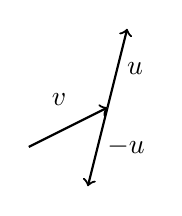
\begin{tikzpicture}
                \draw[->,thick] (0,0)--(1,0.5);
                \draw (0.6,0.6) node[anchor=east] {$v$};
                \draw[->,thick] (1,0.5)--(1.25,1.5);
                \draw (1.125,1) node[anchor=west] {$u$};
                \draw[->,thick] (1,0.5)--(0.75,-0.5);
                \draw (0.875,0) node[anchor=west] {$-u$};
            \end{tikzpicture}
        \end{center}
        
        Thus, if ABCD is a parallelogram with diagonals \( D_1, D_2 \neq 0 \), then
        \begin{align*} \lVert D_1 \rVert^2 = \lVert \overrightarrow{AD} + \overrightarrow{DC} \rVert^2 = &\lVert \overrightarrow{BC} + \overrightarrow{CD} \rVert^2 = \lVert \overrightarrow{AD} - \overrightarrow{DC} \rVert^2 = \lVert D_2 \rVert^2 \\
        &\text{iff} \\
        \overrightarrow{AD} \cdot \overrightarrow{DC} &= 0
        \end{align*}
        which implies the result.
    \end{proof}
\end{exercise} %e1.2.10

\begin{exercise} \label{e1.2.11}
    Use the fundamental properties of the dot product to prove that
    \[ \lVert x+y \rVert^2 + \lVert x-y \rVert^2 = 2\left( \lVert x \rVert^2 + \lVert y \rVert^2 \right)  \]
    
    \begin{proof}
        \begin{align*}
            \lVert x+y \rVert^2 + \lVert x-y \rVert^2 &= (x+y) \cdot (x+y) + (x-y) \cdot (x-y) \\
            &= (x \cdot x) + 2(x \cdot y) + (y \cdot y) + (x \cdot x) - 2(x \cdot y) + (y \cdot y) \\
            &= 2(x \cdot x) + 2 (y \cdot y) \\
            &= 2 \left( \lVert x \rVert^2 + \lVert y \rVert^2 \right)
        \end{align*}
    \end{proof}
\end{exercise} %e1.2.11

\begin{exercise} \label{e1.2.12}
    Use the dot product to prove the law of cosines
    
    \[ c^2 = a^2 + b^2 -2ab\cos{\theta} \]
    
    \begin{center}
        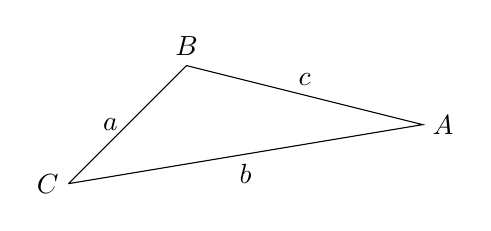
\begin{tikzpicture}
            \draw[] (0,0)
            --(0.75,0.75) node[anchor=east] {$a$}
            --(1.5,1.5) node[anchor=south] {$B$}
            --(3,1.125) node[anchor=south] {$c$}
            --(4.5,0.75) node[anchor=west] {$A$}
            --(2.25,0.375) node[anchor=north] {$b$}
            --(0,0) node[anchor=east] {$C$};
        \end{tikzpicture}
    \end{center}
    
    \begin{proof}
        \begin{align*}
            c^2 &= \lVert \overrightarrow{CA} - \overrightarrow{CB} \rVert^2 \\
            &= (\overrightarrow{CA}-\overrightarrow{CB}) \cdot (\overrightarrow{CA}-\overrightarrow{CB}) \\
            &= \lVert \overrightarrow{CA} \rVert^2 + \lVert \overrightarrow{CB} \rVert^2 - 2\left( \overrightarrow{CA} \cdot \overrightarrow{CB} \right) \\
            &= a^2 + b^2 - 2ab\cos{\theta}
        \end{align*}
    \end{proof}
\end{exercise} %e1.2.12

\begin{exercise} \label{e1.2.13}
    Use vector methods to prove that the diagonals of a parallelogram are orthogonal if and only if the parallelogram is a rhombus (i.e., has all sides of equal length).
    
    \begin{proof}Consider the parallelogram
    
        \begin{center}
            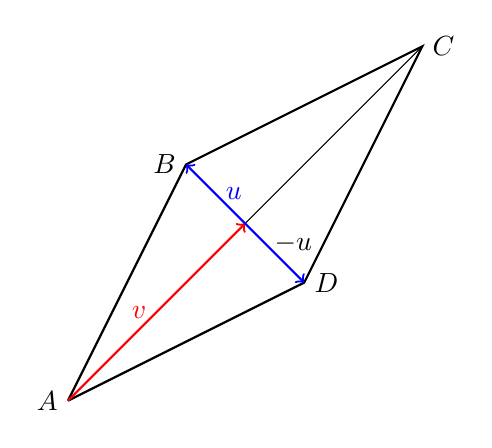
\begin{tikzpicture}
                \draw[thick] (0,0)
                -- (1.5,3) node[anchor=east] {$B$}
                -- (4.5,4.5) node[anchor=west] {$C$}
                -- (3,1.5) node[anchor=west] {$D$}
                -- (0,0) node[anchor=east] {$A$};
                
                \draw (0,0) -- (4.5,4.5);
                \draw (1.5,3) -- (3,1.5);
                
                \draw[->,thick,red] (0,0) 
                -- (1.125,1.125) node[anchor=east] {$v$}
                -- (2.25,2.25);
                
                \draw[->,thick,blue] (2.25,2.25)
                -- (1.875,2.625) node[anchor=west] {$u$}
                -- (1.5,3);
                
                \draw[->,thick,blue] (2.25,2.25)
                -- (2.625,1.875)
                -- (3,1.5);
                
                \draw (2.5,2) node[anchor=west] {$-u$};
            \end{tikzpicture}
        \end{center}
        
        From Exercise \ref{e1.2.10},
        
        \[ \lVert v+u \rVert = \lVert v-u \rVert \text{ iff } v \cdot u = 0 \]
    \end{proof}
\end{exercise} %e1.2.13

\begin{exercise} \label{e1.2.14}
    Use vector methods to prove that a triangle inscribed in a circle and having a diameter as one of the sides must be a right triangle.
    
    \vspace{1cm}
    
    \emph{Geometric Challenge:} More generally, given two points \( A \) and \( B \) in the plane, what is the locus of points \( X \) so that \( \angle AXB \) has a fixed measure?
    
    \begin{proof}
        Note that this is a simple consequence of the inscribed angle theorem. Using vector methods, given
        
        \begin{center}
            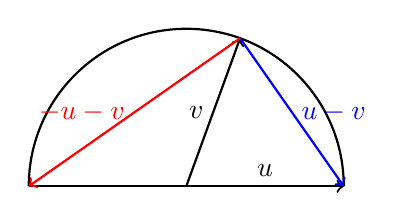
\begin{tikzpicture}
                \draw[thick] (2,0) arc (0:180:2);
                \draw[thick] (-2,0) -- (0,0);
                \draw[thick,->] (0,0) -- (0.684040287,1.879385242);
                \draw[thick,->] (0,0) -- (2,0);
                \draw[->,color=blue,thick] (0.684040287,1.879385242) -- (2,0);
                \draw[->,color=red,thick] (0.684040287,1.879385242) -- (-2,0);
                
                \draw (0.342020143,0.939692621) node[anchor=east] {$v$};
                \draw (1,0) node[anchor=south] {$u$};
                
                \draw[color=blue] (1.342020144,0.939692621) node[anchor=west] {$u-v$};
                \draw[color=red] (-0.657979856,0.939692621) node[anchor=east] {$-u-v$};
            \end{tikzpicture}
        \end{center}
        
        \noindent Note \( \lVert v \rVert = \lVert u \rVert \). It follows 
        \[ (u-v) \cdot (-u-v) = -\lVert u \rVert^2 + \lVert v \rVert^2 = 0\]
        implying the result.
        
        \vspace{1cm}
        
        \emph{Geometric Challenge:} Suppose \( X \) is chosen so that \( \angle AXB = \theta \). Then
        \begin{center}
            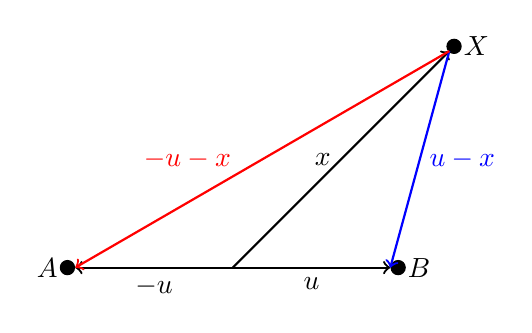
\begin{tikzpicture}
                \draw[thick, ->] (0,0) -- (-2,0);
                \draw[thick, ->] (0,0) -- (2,0);
                
                \draw (-2.1,0) node[anchor=east] {$A$};
                \draw[fill=black] (-2.1,0) circle(0.09);
                
                \draw (2.1,0) node[anchor=west] {$B$};
                \draw[fill=black] (2.1,0) circle(0.09);
                
                \draw (-1,0) node[anchor=north] {$-u$};
                \draw (1,0) node[anchor=north] {$u$};
                
                \draw[thick, ->] (0,0) -- (1.375,1.375) node[anchor=east] {$x$} -- (2.75,2.75);
                
                \draw (2.81,2.81) node[anchor=west] {$X$};
                \draw[fill=black] (2.81,2.81) circle(0.09);
                
                \draw[thick,color=blue,->] (2.75,2.75) -- (2,0);
                \draw[thick,color=red,->] (2.75,2.75) -- (-2,0);
                
                \draw[color=blue] (2.375,1.375) node[anchor=west] {$u-x$};
                \draw[color=red] (0.1,1.375) node[anchor=east] {$-u-x$};
            \end{tikzpicture}
        \end{center}
        
        So that
        \[ \cos{\theta} = \frac{(u-x) \cdot (-u-x)}{\lVert u-x \rVert \lVert u+x \rVert} = \frac{\lVert x \rVert^2 - \lVert u \rVert^2}{\lVert u-x \rVert \lVert u+x \rVert} \]
        
        which defines our locus.
    \end{proof}
\end{exercise} %e1.2.14
\subsection{Subspaces of $\mathbb{R}^n$}

\subsection{Linear Transformations and Matrix Algebra}

\subsection{Introduction to Determinants and the Cross Product}


\newpage
\section{FUNCTIONS, LIMITS, AND CONTINUITY}

\subsection{Scalar and Vector-Valued Functions}

\subsection{A Bit of Topology in \( \mathbb{R}^n \)}

\subsection{Limits and Continuity}


\newpage
\section{THE DERIVATIVE}
\subsection{Partial Derivatives and Directional Derivatives}

\subsection{Differentiability}

\subsection{Differentiation Rules}

\subsection{The Gradient}

\subsection{Curves}

\subsection{Higher-Order Partial Derivatives}


\newpage
\section{IMPLICIT AND EXPLICIT SOLUTIONS OF LINEAR SYSTEMS}
\subsection{Gaussian Elimination and the Theory of Linear Systems}
\subsection{Elementary Matrices and Calculating Inverse Matrices}
\subsection{Linear Independence, Basis, and Dimensions}
\subsection{The Four Fundamental Subspaces}
\subsection{The Nonlinear Case: Introduction to Manifolds}


\newpage
\section{IMPLICIT AND EXPLICIT SOLUTIONS OF LINEAR SYSTEMS}
\subsection{Gaussian Elimination and the Theory of Linear Systems}
\subsection{Elementary Matrices and Calculating Inverse Matrices}
\subsection{Linear Independence, Basis, and Dimensions}
\subsection{The Four Fundamental Subspaces}
\subsection{The Nonlinear Case: Introduction to Manifolds}


\newpage
\section{EXTREMUM PROBLEMS}
\subsection{Compactness}
\subsection{Maximum/Minimum Problems}
\subsection{Quadratic Forms and the Second Derivative Test}
\subsection{Lagrange Multipliers}
\subsection{Projections, Lease Squares, and Inner Product Spaces}


\newpage
\section{SOLVING NONLINEAR PROBLEMS}
\subsection{The Contraction Mapping Principle}
\subsection{The Inverse and Implicit Function Theorems}
\subsection{Manifolds Revisited}


\newpage
\section{INTEGRATION}
\subsection{Multiple Integrals}
\subsection{Iterated Integrals and Fubini's Theorem}
\subsection{Polar, Cylindrical, and Spherical Coordinates}
\subsection{Physical Applications}
\subsection{Determinants and $n$-Dimensional Volume}
\subsection{Chabnge of Variables Theorem}


\newpage
\section{DIFFERENTIAL FORMS AND INTEGRATION ON MANIFOLDS}
\subsection{Motivation}
\subsection{Differential Forms}
\subsection{Line Integrals and Green's Theorem}
\subsection{Surface Integrals and Flux}
\subsection{Stokes' Theorem}
\subsection{Applications to Physics}
\subsection{Applications to Topology}


\newpage
\section{EIGENVALUES, EIGENVECTORS, AND APPLICATIONS}
\subsection{Linear Transformations and Change of Basis}
\subsection{Eigenvalues, Eigenvectors, and Diagonalizability}
\subsection{Difference Equations and Ordinary Differential Equations}
\subsection{The Spectral Theorem}


\end{document}
